\documentclass[hyperref={pdfpagelabel=false},usepdftitle=false,xcolor=dvipsnames]{beamer}

\usepackage[T1]{fontenc}
\usepackage[utf8]{inputenc}
\usepackage[russian]{babel}

\usepackage{amssymb, amsmath}

\usepackage{subfig}
%\usepackage{subcaption}

\usepackage{tikz}
\usetikzlibrary{shapes.geometric, arrows, positioning, decorations.markings}
\usetikzlibrary{fit}
\usepackage{microtype}
\usepackage{framed}
\usetikzlibrary{decorations.pathmorphing,calc,backgrounds}

\usetheme{CambridgeUS}
\useinnertheme{rectangles}
\useoutertheme{infolines}

\setbeamercolor{frametitle}{fg=Brown, bg = Brown!20}

\title{\textbf{Поль Сабатье \\ 5.XI.1854 - 14.VIII.1941}}

\author{\small
\begin{flushright}
Выполнил: Финенко А. А. \\ 515 группа \\[15ex]
\end{flushright}
}

\pdfmapfile{+sansmathaccent.map}

\institute[MSU] % (optional, but mostly needed)
{\small МГУ им. М.В.Ломоносова, Химический факультет, 2017}
\date{}

\newcommand\Fontvi{\fontsize{6}{7.2}\selectfont}

\beamertemplatenavigationsymbolsempty

\setbeamerfont{page number in head/foot}{size=\large}
\setbeamertemplate{footline}[frame number]
\setbeamertemplate{frametitle}[default][center]

% change font
\usefonttheme[onlymath]{serif}

\makeatother
\setbeamertemplate{headline}
{}
\makeatletter

\makeatother
\setbeamertemplate{footline}
{
  \leavevmode%
  \hbox{%
  \begin{beamercolorbox}[wd=.7\paperwidth,ht=2.25ex,dp=1ex,center]{author in head/foot}%
    \usebeamerfont{author in head/foot} Поль Сабатье 
  \end{beamercolorbox}%
	\begin{beamercolorbox}[wd=.3\paperwidth,ht=2.25ex,dp=1ex,center]{title in head/foot}%
    \usebeamerfont{title in head/foot}Финенко А. \hspace*{3em}
    \insertframenumber{} / \inserttotalframenumber\hspace*{1ex}
  \end{beamercolorbox}}%
  \vskip0pt%
}
\makeatletter
\setbeamertemplate{navigation symbols}{}

\begin{document}

\begin{frame}
{
\vspace*{-0.75cm}
\large 
\begin{center}
Кафедра физической химии \\
Лаборатория строения и квантовой механики молекул
\vspace*{-0.75cm}
\end{center}}
 \titlepage
\end{frame}

\begin{frame}{Ранние годы I}
Он родился 5 ноября 1854 года в Каркассоне в Южной Франции. Его родители -- Полина (Гилам) Сабатье и Алексис Сабатье. Семейство Сабатье вскоре после рождения Поля разорилась и лишилась собственности из-за неуплаты налогов. Благодаря помощи друзей семьи Алексис Сабатье открыл шляпный магазин. Поль был одним из трех сыновей и младшим ребенком в семье, состоявшей из семи детей. 
\begin{figure}	
	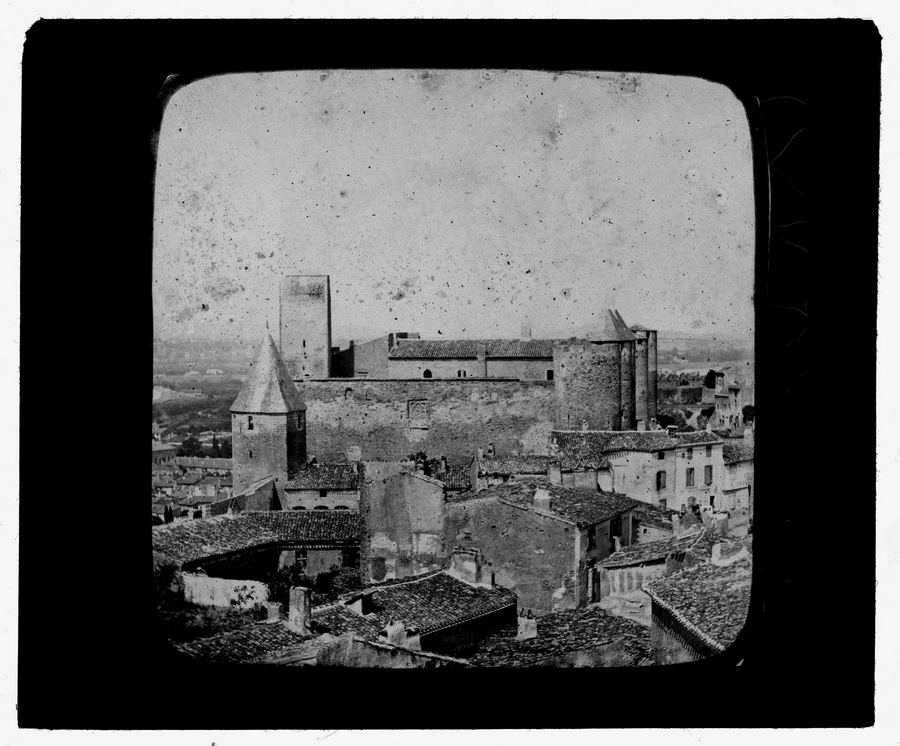
\includegraphics[width=0.37\linewidth]{pictures/carcassone1.jpg}
	\hspace{0.2cm}
	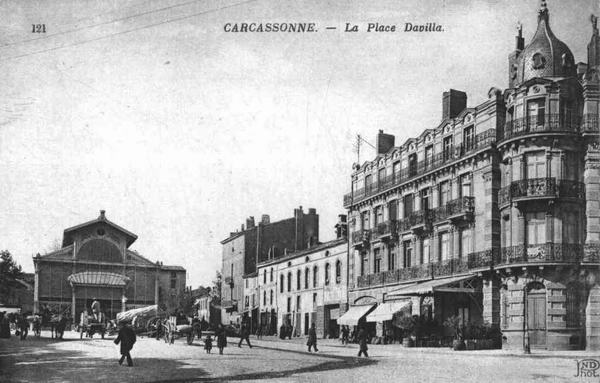
\includegraphics[width=0.48\linewidth]{pictures/carcassone2.jpg}
	\caption{Вид замка Каркассон в конце 19 века (слева)[1]; главная площадь Каркассона (справа)[2]}
\end{figure}

\end{frame}

\begin{frame}{Ранние годы II}
В 1868 г. Поль перешел в тулузский лицей, чтобы готовиться к вступительным экзаменам в университет. В Тулузе посещал публичные лекции по физике и химии, которые пробудили в нем желание заниматься научными исследованиями. В 1874 г. он занял первое место на вступительных экзаменах и поступил в Политехническую школу. 
\begin{figure}
	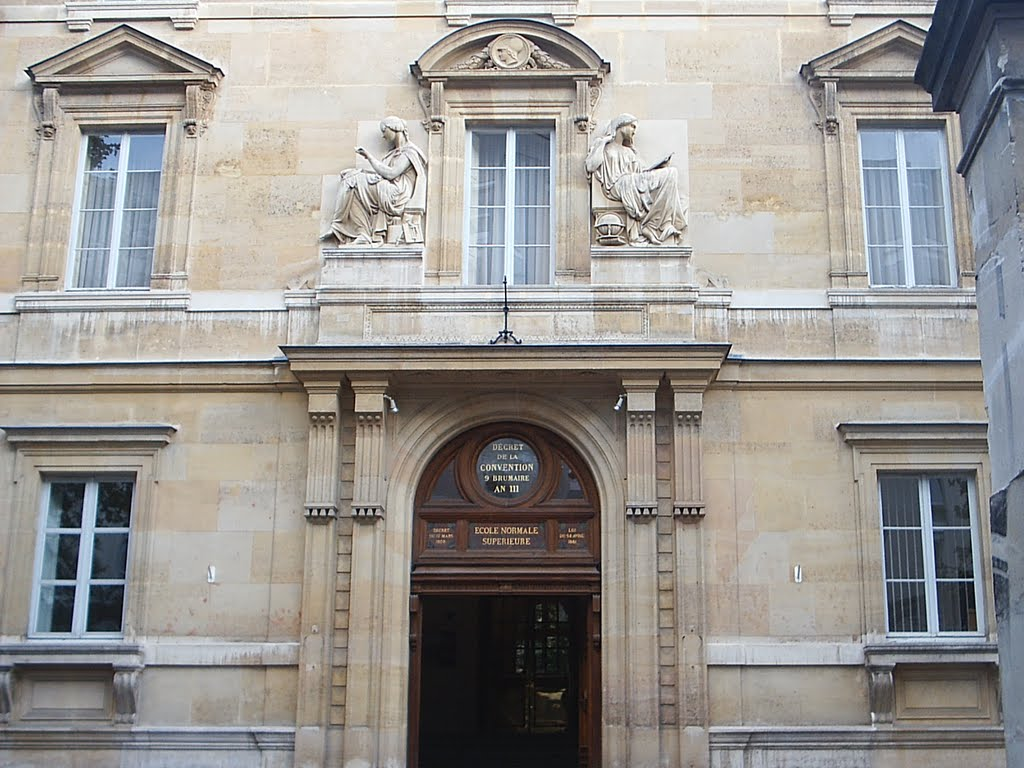
\includegraphics[width=0.48\linewidth]{pictures/ens1.jpg}
	\caption{\centering Здание Политехнической школы в Париже [3]}
		\end{figure}
\end{frame}

\begin{frame}{Ранние годы III}
	Спустя три года закончил Политехническую школу, будучи лучшим студентом в группе. В течение следующего года он преподавал физику в лицее в Ниме. 
	\begin{figure}
		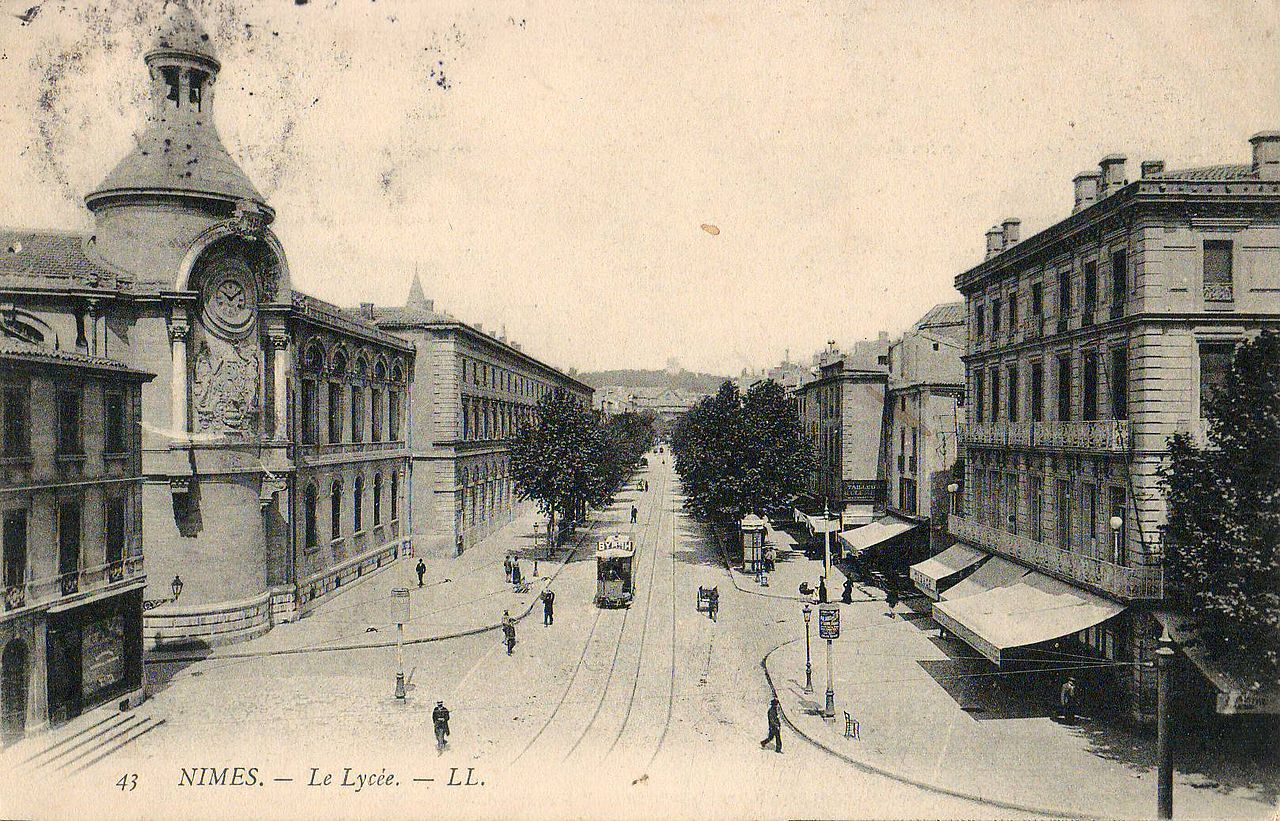
\includegraphics[width=0.47\linewidth]{pictures/nimes.jpg}
		\hspace{0.2cm}
		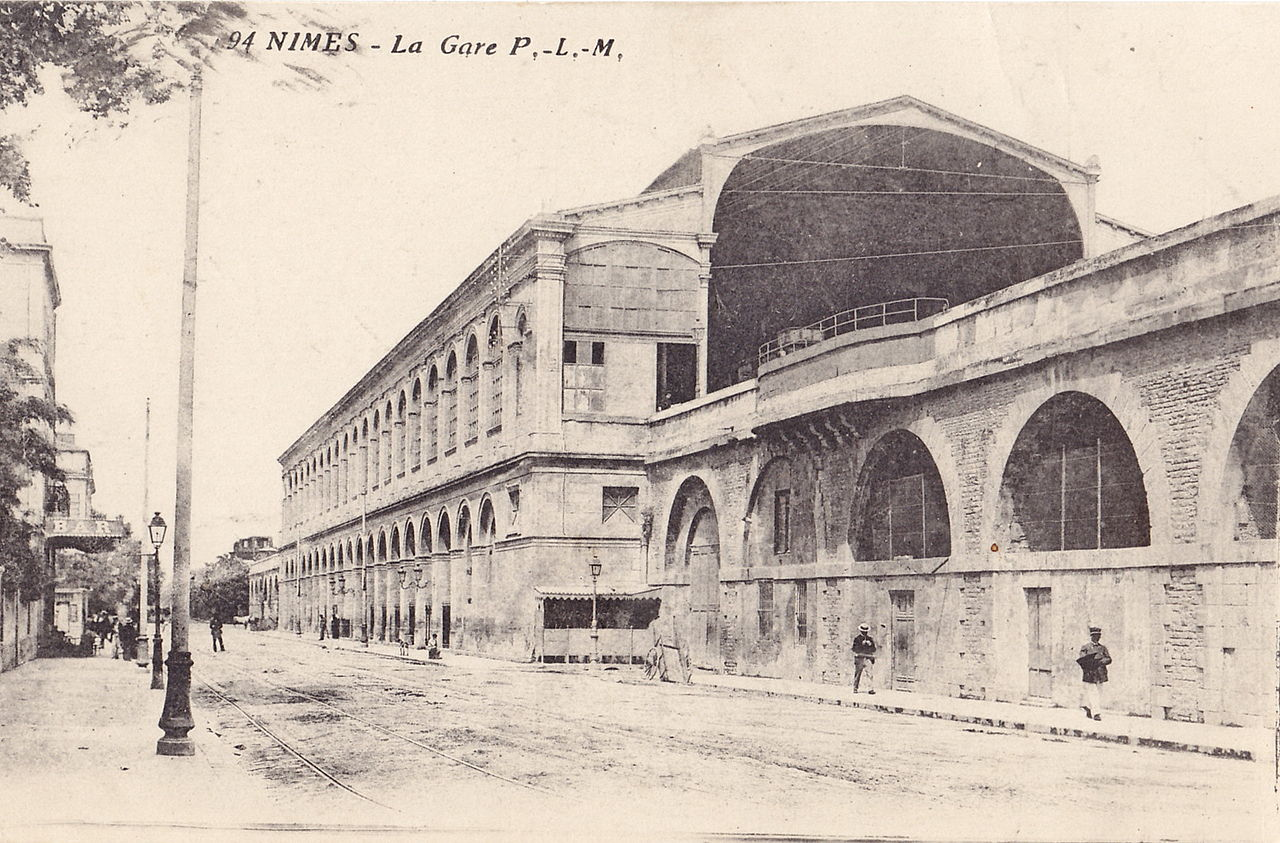
\includegraphics[width=0.47\linewidth]{pictures/nimes2.jpg}
		\caption{\centering Вокзал в Ниме до 1839 г. (слева)[4], трамвайная станция в Ниме в 1880-1951 гг. (справа)[4]}
	\end{figure}
\end{frame}

\begin{frame}{Научная карьера I}
	В 1878-1880 работал ассистентом у П. Э. М. Бертло в Коллеж де Франс в Париже. По итогам работы в 1880 Сабатье получил докторскую степень за диссертацию по тематике термохимических свойств серы и сульфатов. 
	\begin{columns}
	\begin{column}{0.5\linewidth}
	\begin{figure}
		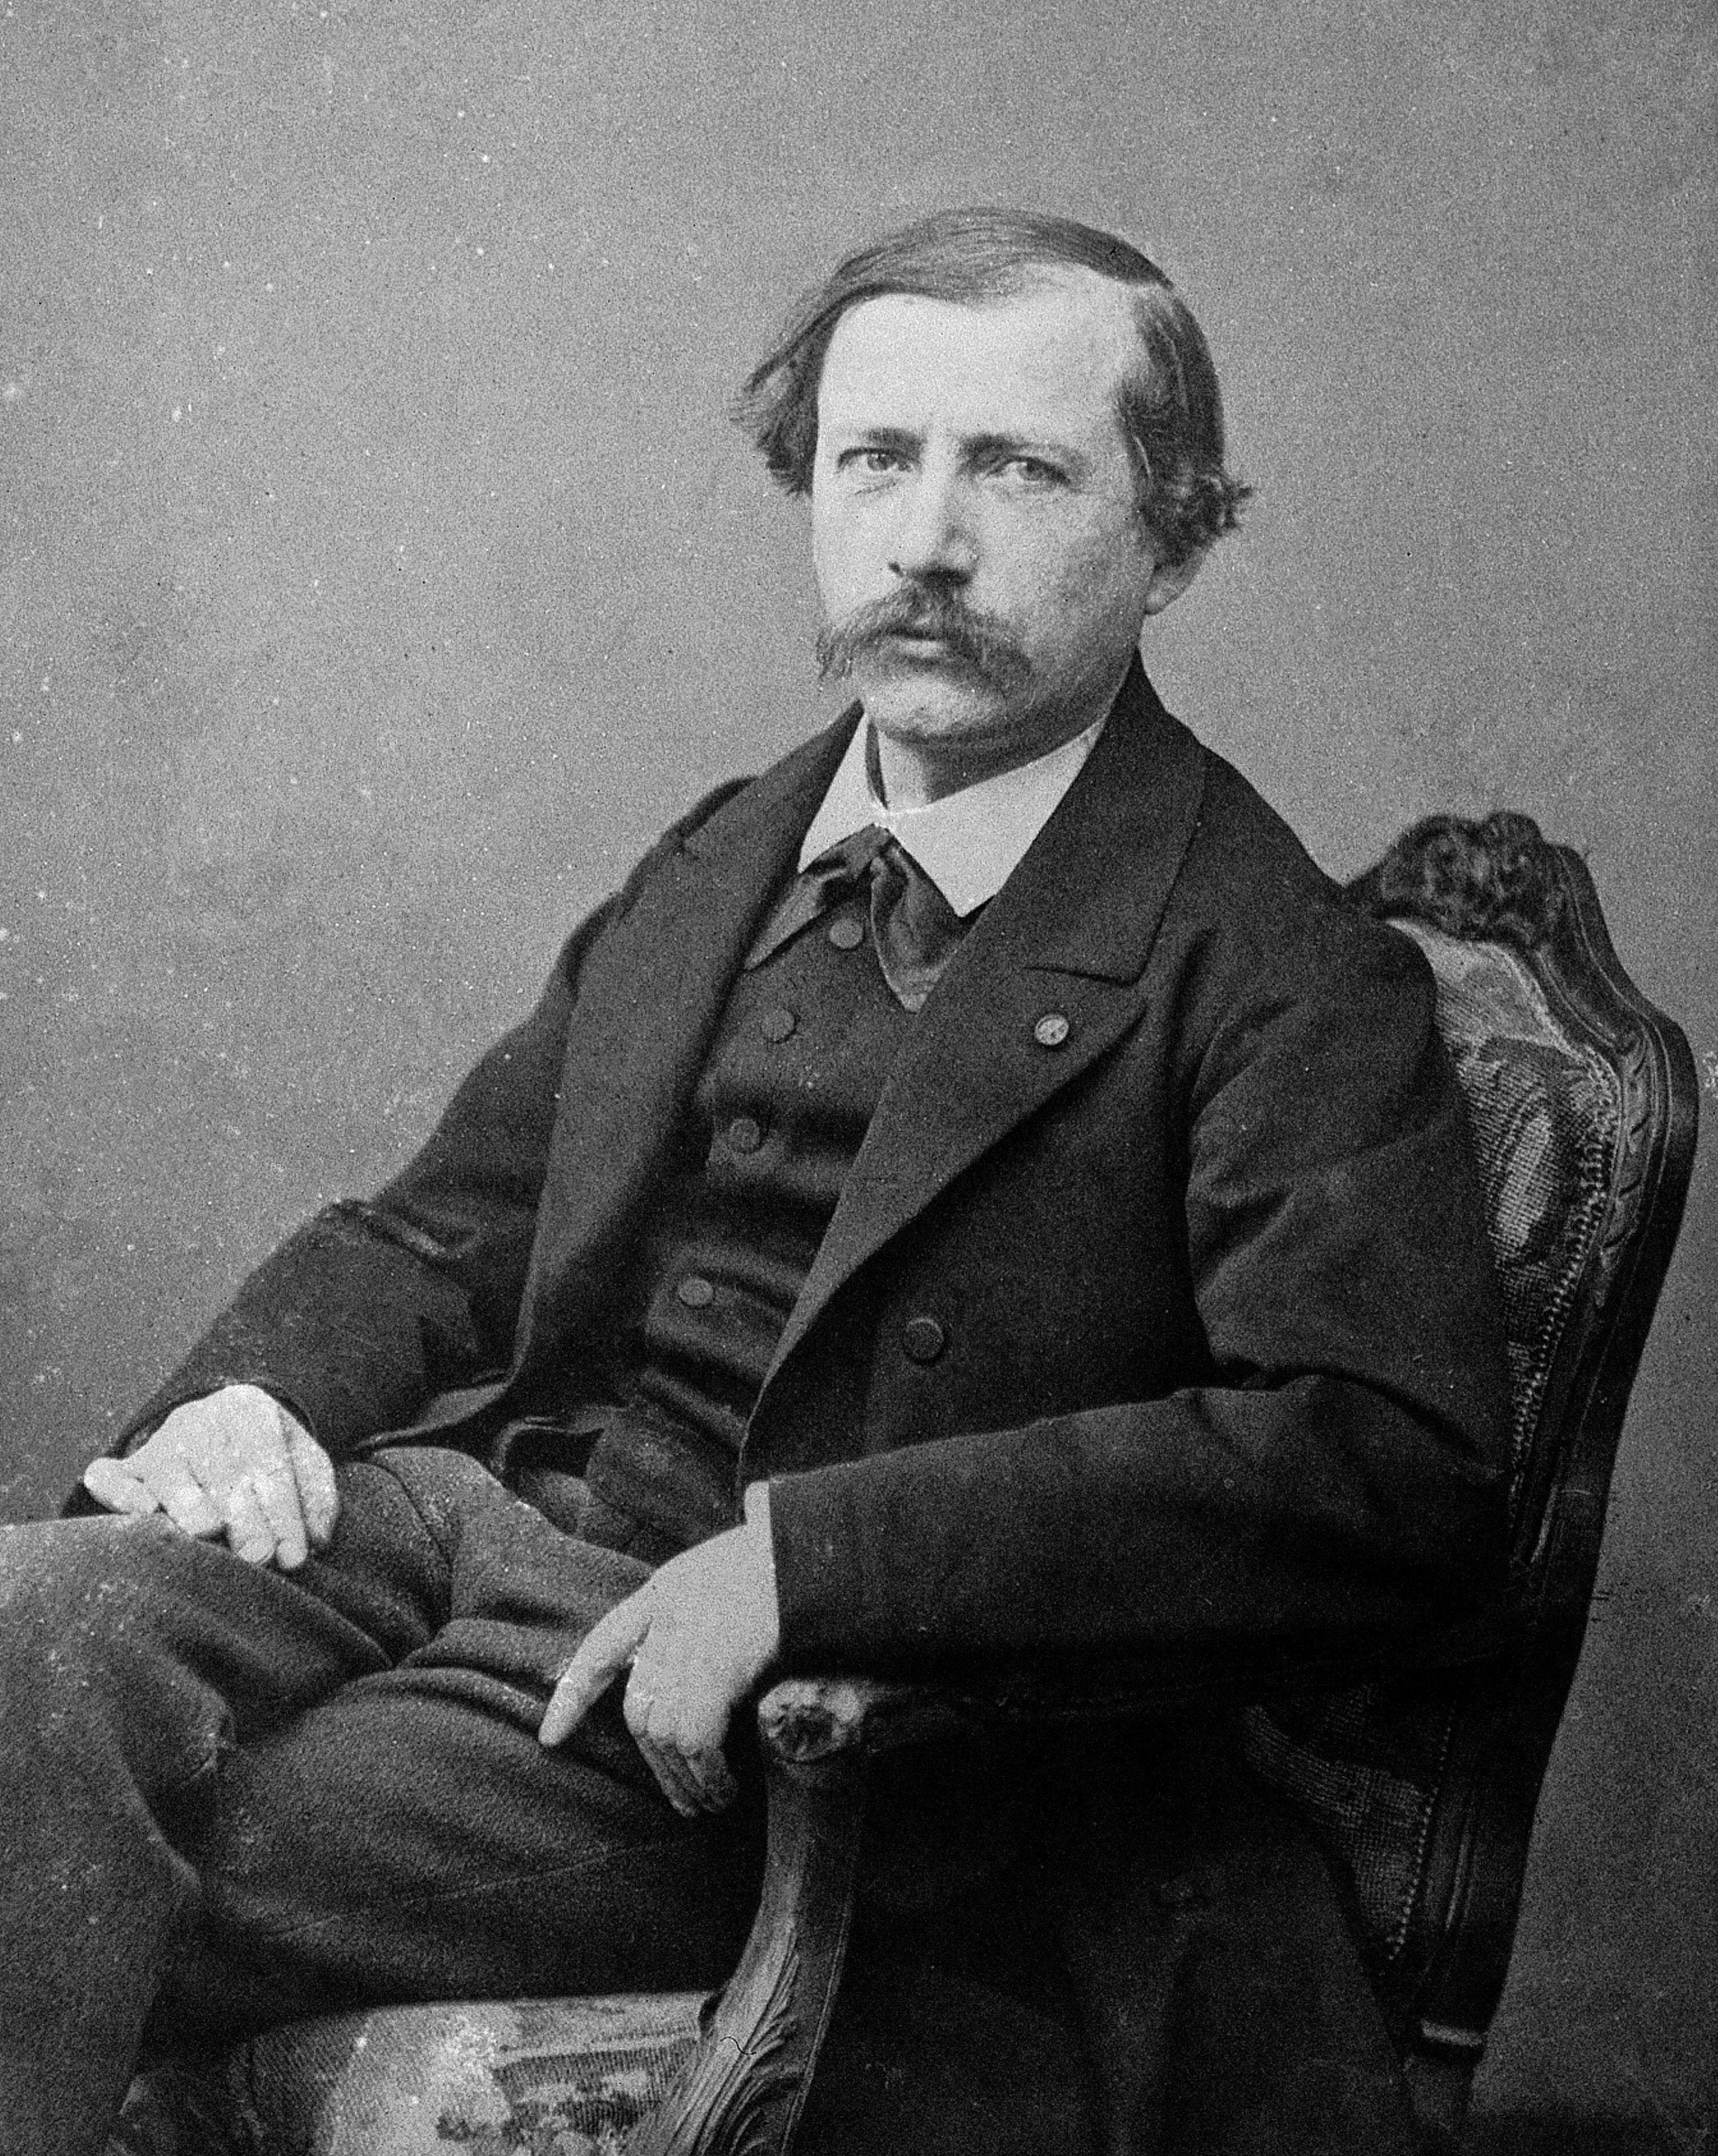
\includegraphics[width=0.6\linewidth]{pictures/berthelot.jpg}
		\caption{П. Э. М. Бертло[5]}
	\end{figure}
	\end{column}
	\begin{column}{0.5\linewidth}
		В течение следующего года П. Сабатье изучал физику в университете Бордо. В 1884 г. он вернулся в Тулузу и возглавил кафедру химии Тулузского университета, которую возглавлял до конца своей научной карьеры. 
	\end{column}
	\end{columns}
\end{frame}

\begin{frame}{Научная карьера II}
		В 1905 г. П. Сабатье был назначен деканом факультета, в 1907 г. получил приглашение занять место Анри Муассана в университете Сорбонне, но предпочел остаться в Тулузе. 
	\begin{figure}
		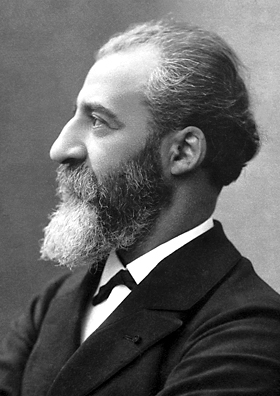
\includegraphics[width = 0.32\linewidth]{pictures/moissan.jpg}
		\hspace{0.2cm}
		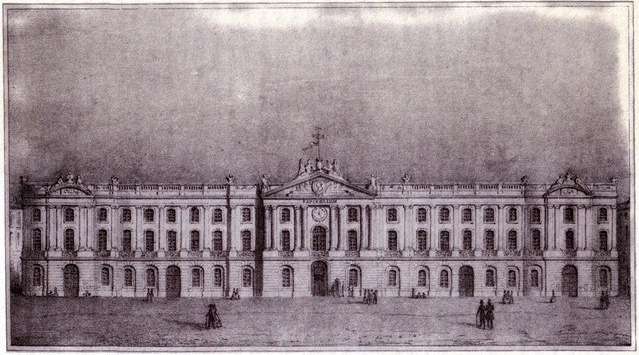
\includegraphics[width=0.5\linewidth, height = 3.75cm]{pictures/capitole.png}
		\caption{Анри Муассан (слева)[6]; главное здание Тулузского университета (справа)[7]}
	\end{figure}
\end{frame}

\begin{frame}{Научная карьера III}
	П. Сабатье внес неоценимый вклад в неорганическую химию, но мировая известность пришла к нему за работы в области гетерогенного катализа. В 1897 г. П. Сабатье начал сотрудничество с Ж. Б. Сендереном. Изначально, их исследования касались гидрогенирования ненасыщенных углеводородов, катализируемого оксидами металлов. Впоследствии исследования сосредоточились конкретно на использовании никеля и его оксида в качестве катализатора реакции гидрогенирования.
\begin{figure}
	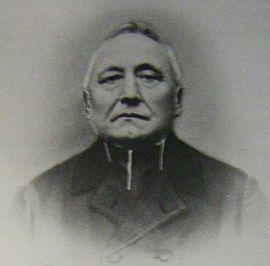
\includegraphics[width = 0.27\linewidth]{pictures/senderens.jpg}
	\caption{Жан-Батист Сендеренс[8]}
\end{figure}
\end{frame}

\begin{frame}{Научная карьера IV}
		Особенно стоит отметить работы П. Сабатье по следующим тематикам: гидрогенирование бензола и его гомологов (1901), восстановление простейших альдегидов и кетонов (1902-1903), каталитическая конверсия спиртов под действиемметаллов (1907-1911), гидрогенирование ненансыщенных карбоновых кислот (1909). В 1913 году Сабатье подвел итог своим исследованиям в области катализа, выпустив монографию \textit{La catalyse en chimie organique} (Paris, 1913).
\begin{figure}
	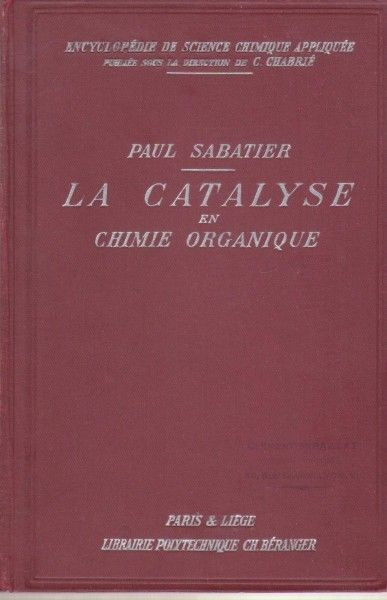
\includegraphics[width=0.2\linewidth]{pictures/book.jpg}
	\caption{Монография П. Сабатье \textit{La catalyse en chimie organique}[9]}
\end{figure}
\end{frame}

\begin{frame}{Сотрудничество с Ипатьевым}
	В 1900 г. один из самых выдающихся химиков первой половины XX века, В. Н. Ипатьев, начал исследования в области гетерогенного катализа органических реакций. Схожесть интересов и научных целей Сабатье и Ипатьева привели к долговременному сотрудничеству. 
	\begin{figure}
		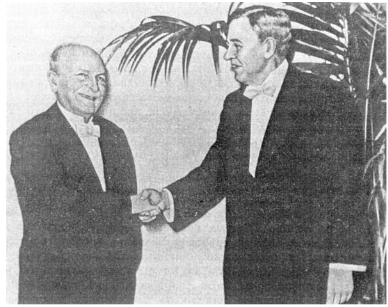
\includegraphics[width = 0.5\linewidth]{pictures/ipatiev.png}
		\caption{П. Сабатье (слева) и В. Н. Ипатьев (справа), Париж, 1936 [10]}
	\end{figure}
\end{frame}


\begin{frame}{Научное признание I}
		\begin{columns}
\begin{column}{0.4\textwidth}
\begin{figure}
	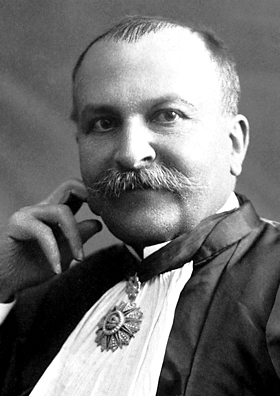
\includegraphics[width=0.8\linewidth]{pictures/sabatier.jpg}
	\caption{П. Сабатье [11]}
\end{figure}
\end{column}
\begin{column}{0.6\linewidth}
		Еще в 1907 году исследования П. Сабатье по каталитическому гидрогенированию были высоко оценены научным сообществом, и он был номинирован для получения Нобелевской Премии в 1907, 1909 и 1911 годах. В 1909 году, ближайший коллега Сабатье Ж. Б. Сендеренс, также был среди номинантов. Нобелевская Премия была присуждена П. Сабатье в 1912 г. (и В. Гриньяру) со следующей формулировкой: \textit{"за метод гидрогенирования органических соединений в присутствии мелко измельченных металлов, вследствие чего органическая химия достигла существенно прогресса"}. 
\end{column}
\end{columns}
\end{frame}

\begin{frame}{Научное признание II}
	В 1929 г. Сабатье ушел с должности декана факультета в Тулузском университете, а в на следующий год подал в отставку. Однако до самого конца жизни он продолжал читать лекции в различных научных учреждениях по всему миру. Академии и научные сообщества выбирали его в качестве почетного иностранного члена. Помимо Нобелевской премии, Сабатье получил премию Джекера Французской академии наук (1905), медаль Дэви (1915) и Королевскую медаль (1918) Лондонского королевского общества, а также медаль Франклина (1933). Он являлся членом Французской академии наук, иностранным членом Лондонского королевского общества, Мадридской академии наук, Нидерланской королевской академии наук, Американского химического общества и многих других.
\end{frame}

\begin{frame}{Личная жизнь}
	\begin{columns}
	\begin{column}{0.5\linewidth}
		\begin{figure}
			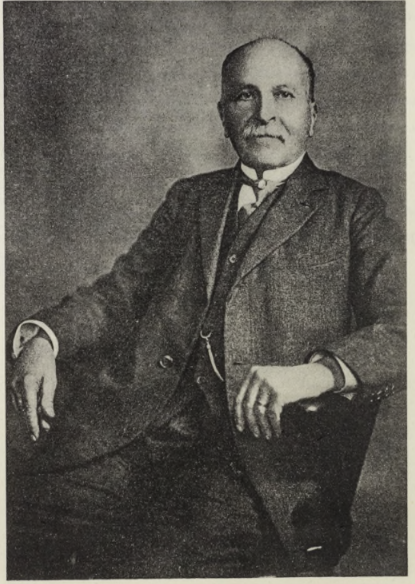
\includegraphics[width = 0.75\linewidth]{pictures/sabatier2.png}
			\caption{П. Сабатье [12]}
		\end{figure}
	\end{column}
	\begin{column}{0.5\linewidth}
			В 1884 г. П. Сабатье соединил свою судьбу с Жермен Эраль, дочерью местного судьи. У них родились четыре дочери. После смерти жены в 1898 г. Сабатье никогда больше не женился. Одна из его дочерей вышла замуж за химика итальянского происхождения Эмилио Помилио. Сабатье ушел из жизни 14 августа 1941 г. в Тулузе.
	\end{column}
	\end{columns}
\end{frame}

\begin{frame}{Наследие}
	Университет в Тулузе получил имя Поля Сабатье. П. Сабатье вместе с Т. Ж. Стилтьесом и др. стали сооснователями научного журнала \textit{Annales de la Faculte des Sciences de Toulouse}.
	\begin{figure}
		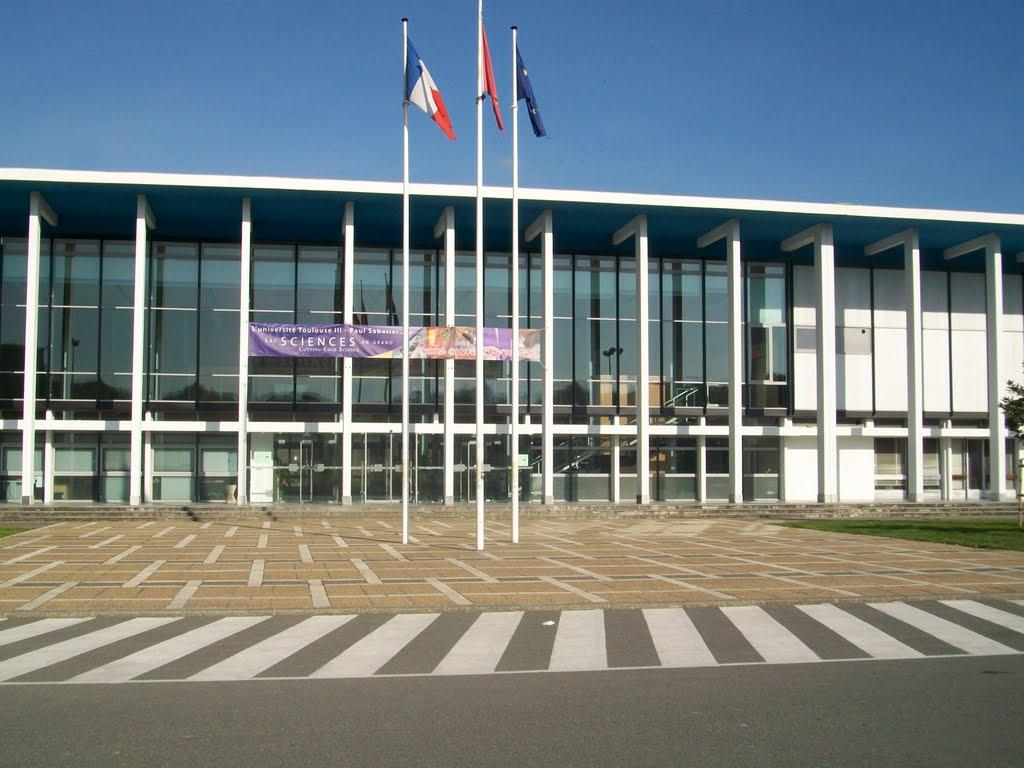
\includegraphics[width=0.5\linewidth]{pictures/university.jpeg}
		
\includegraphics[width=0.5\linewidth]{pictures/university2.jpeg}
		\caption{Современная фотография университета Поля Сабатье в Тулузе (слева)[13], эмблема университета (справа)[14]}
	\end{figure}
\end{frame}

\begin{frame}{Список использованной литературы I}
	\begin{block}{i. Литературные источники биографического характера}
	\begin{enumerate}
			\item Morachevskii, A. G. (2004). \textit{Russ. J. Appl. Chem.}, \textbf{77}.
			\item Rideal, E. K. (1951). Presidential address. Concepts in catalysis. The contributions of Paul Sabatier and of Max Bodenstein. \textit{J. Chem. Soc. (Resumed)}: 1640–1647.
			\item Taylor, H. (1944). Paul Sabatier 1854–1941. \textit{J. Am. Chem. Soc.}. \textbf{66} (10): 1615–1617.
			\item Bykov, G.V. Istoriya organicheskoi khimii (History of Organic Chemistry), Moscow: Nauka, 1978.
			\item Волков, В.А., Вонский, Е. В., Кузнецова, Г. И. Выдающиеся химики мира. Биографический справочник. Москва: Высшая школа. 1991
			\item https://www.thefamouspeople.com/profiles/paul-sabatier-7149.php
			\item https://hu.wikipedia.org/wiki/Paul-Sabatier 
	\end{enumerate}
	\end{block}
\end{frame}

\begin{frame}{Список используемой литературы II}
		\begin{block}{ii. Ссылки на источники иллюстраций}
			\begin{enumerate}
				\item https://en.wikipedia.org/wiki/Carcassonne
				\item https://fr.wikipedia.org/wiki/Carcassonne
				\item http://www.panoramio.com/photo/ 
				\item https://fr.wikipedia.org/wiki/Nimes
				\item https://en.wikipedia.org/wiki/Marcellin-Berthelot
				\item https://en.wikipedia.org/wiki/Henri-Moissan 
				\item http://www.alamy.com/
				\item https://nl.wikipedia.org/wiki/Jean-Baptiste-Senderens
				\item https://catalog.hathitrust.org/ 
			\end{enumerate}
		\end{block}
\end{frame}

\begin{frame}{Список используемой литературы III}
	\begin{block}{iii. Ссылки на источники иллюстраций}
		\begin{enumerate}
			\setcounter{enumi}{9}	
			\item Morachevskii, A. G. (2004). \textit{Russ. J. Appl. Chem.}, \textbf{77}.
			\item https://en.wikipedia.org/wiki/Paul-Sabatier-(chemist) 
			\item Rideal, E. K. (1951). Presidential address. Concepts in catalysis. The contributions of Paul Sabatier and of Max Bodenstein. \textit{J. Chem. Soc. (Resumed)}: 1640–1647.
			\item https://www.unipage.net/en/610/paul-sabatier-university
			\item https://www.unipage.net/en/610/paul-sabatier-university 
		\end{enumerate}
	\end{block}
\end{frame}

\end{document}





